\section{Main Learning Paradigms}

So far, learning has been described through a common mathematical language: data, hypothesis classes, losses, risk, and optimization. But not all learning problems present information in the same way. In some settings the learner receives explicit labels; in others it must discover structure from raw observations; in still others it must act, observe consequences, and improve through delayed feedback.

These differences give rise to the main paradigms of machine learning. The point of this section is not merely to list them, but to unify them. The paradigms differ in the form of supervision they provide, yet all can be viewed as optimizing objective functionals built from data or interaction.

\subsection*{Four supervision regimes}

\begin{definition}[Supervised learning]
In \emph{supervised learning}, the learner receives examples of the form
\[
(x_i,y_i)\in \mathcal X\times \mathcal Y,
\]
where $x_i$ is an input and $y_i$ is a target or label. The goal is to learn a predictor
\[
f:\mathcal X\to\mathcal Y
\]
that performs well on future labeled examples.
\end{definition}

The supervision signal here is explicit: the desired output is provided directly by the data source.

\begin{definition}[Unsupervised learning]
In \emph{unsupervised learning}, the learner observes inputs
\[
x_1,\dots,x_n\in\mathcal X
\]
without externally supplied labels. The goal is to discover structure in the data, such as clustering, latent factors, low-dimensional representations, or a model of the data distribution itself.
\end{definition}

The absence of labels does not mean the absence of a task. It means that the task is defined through structure rather than through externally supplied targets.

\begin{definition}[Self-supervised learning]
In \emph{self-supervised learning}, the learner constructs supervision from the data themselves. From raw observations $x$, it defines auxiliary prediction tasks whose targets are derived automatically from the observed sample.
\end{definition}

Examples include predicting a masked token in a sentence, predicting whether two views came from the same image, or reconstructing a withheld part of a signal. The targets are not given by a human annotator, but they are still targets.

\begin{definition}[Reinforcement learning]
In \emph{reinforcement learning}, the learner interacts with an environment over time. At step $t$, it observes a state $s_t$, chooses an action $a_t$, receives a reward $r_t$, and transitions to a new state. The goal is to learn a policy
\[
\pi(a\mid s)
\]
that maximizes expected cumulative reward.
\end{definition}

Here the supervision signal is evaluative rather than corrective: the learner is not told the right action directly, but is told how good the consequences of its behavior were.

\subsection*{A unified optimization viewpoint}

Although these paradigms look different on the surface, they share a common mathematical pattern.

\begin{proposition}[Learning paradigms as objective-based optimization]
Each of the four paradigms can be viewed as selecting an object $h$ from a hypothesis space $\mathcal H$ in order to optimize an objective functional built from observations or interaction:
\[
h^\star \in \arg\min_{h\in\mathcal H} \mathcal J(h)
\qquad\text{or}\qquad
h^\star \in \arg\max_{h\in\mathcal H} \mathcal J(h).
\]
More specifically:
\begin{enumerate}
    \item in supervised learning, $\mathcal J$ is typically an expected prediction loss over labeled pairs $(X,Y)$;
    \item in unsupervised learning, $\mathcal J$ measures a structural criterion over inputs $X$, such as likelihood, reconstruction quality, or clustering distortion;
    \item in self-supervised learning, $\mathcal J$ measures predictive performance on targets automatically derived from raw data;
    \item in reinforcement learning, $\mathcal J$ is expected cumulative reward over trajectories induced by interaction with an environment.
\end{enumerate}
\end{proposition}

\begin{proof}
We verify the claim by writing a representative objective for each regime.

In supervised learning, one often minimizes
\[
\mathcal J(f)=\mathbb E[\ell(f(X),Y)].
\]

In unsupervised learning, one may maximize log-likelihood
\[
\mathcal J(g)=\mathbb E[\log p_g(X)],
\]
or minimize reconstruction error
\[
\mathcal J(g,\phi)=\mathbb E[\|X-g(\phi(X))\|^2].
\]

In self-supervised learning, one defines a target transformation $t(X)$ or paired views derived from $X$ and optimizes an objective such as
\[
\mathcal J(h)=\mathbb E[\ell(h(\tilde X), t(X))].
\]

In reinforcement learning, one optimizes
\[
\mathcal J(\pi)=\mathbb E_\pi\!\left[\sum_{t=0}^\infty \gamma^t r_t\right],
\]
where the expectation is over trajectories generated by policy $\pi$ and the environment dynamics.

Thus, despite differing forms of supervision, each paradigm is governed by an objective functional over data or interaction.
\end{proof}

This proposition is important because it prevents the chapter from fragmenting into unrelated categories. The paradigms differ in what information is available and what must be predicted or optimized, but they all fit into the broader view of learning as structured objective optimization.

\subsection*{Supervised learning}

Supervised learning is the most direct regime. The learner sees examples together with desired outputs and tries to infer a rule that extends beyond the sample.

Typical tasks include classification and regression. A standard objective is empirical risk minimization:
\[
\hat f \in \arg\min_{f\in\mathcal H} \frac1n\sum_{i=1}^n \ell(f(x_i),y_i).
\]

Its central challenge is generalization: how to use finitely many labeled examples to perform well on new ones.

\subsection*{Unsupervised learning}

In unsupervised learning, the learner receives only raw observations. The aim may be to model the distribution of the data, compress them into a lower-dimensional representation, cluster them into groups, or extract latent structure.

Representative objectives include
\[
\max_\theta \sum_{i=1}^n \log p_\theta(x_i)
\]
for density modeling, or
\[
\min_{\phi,g} \sum_{i=1}^n \|x_i-g(\phi(x_i))\|^2
\]
for autoencoding.

\commonconfusion{``Unsupervised'' does not mean ``no objective.'' It means ``no externally supplied labels.'' Unsupervised methods still optimize clearly defined criteria such as likelihood, reconstruction error, contrastive structure, or clustering distortion.}

\subsection*{Self-supervised learning}

Self-supervised learning occupies a middle ground between supervised and unsupervised learning. It uses raw data, like unsupervised learning, but formulates predictive tasks with explicit targets, like supervised learning.

For example, if $x$ is a sentence and one token is masked, the learner may try to predict the missing token:
\[
\min_\theta \mathbb E[-\log p_\theta(x_j \mid x_{\setminus j})].
\]
If $x$ is an image, the learner may form two transformed views $v_1(x)$ and $v_2(x)$ and train representations so that matching views are close while mismatched views are separated.

The key point is that supervision is \emph{constructed}, not externally annotated.

\commonconfusion{Self-supervised learning is not just unsupervised learning with a fashionable name. Its defining feature is that it creates explicit predictive targets from the data themselves. The model is trained to solve auxiliary prediction tasks, often in ways that produce useful transferable representations.}

\subsection*{Reinforcement learning}

Reinforcement learning differs from the previous regimes because learning occurs through sequential interaction. The learner does not merely observe a static sample; it acts in an environment and experiences the consequences of those actions over time.

A policy $\pi$ is evaluated by expected return
\[
J(\pi)=\mathbb E_\pi\!\left[\sum_{t=0}^\infty \gamma^t r_t\right].
\]
The learner seeks
\[
\pi^\star \in \arg\max_\pi J(\pi).
\]

This introduces new difficulties absent from static prediction:
\begin{itemize}
    \item actions influence future data,
    \item rewards may be delayed,
    \item exploration is necessary,
    \item feedback is often sparse and noisy.
\end{itemize}

Thus reinforcement learning is not merely supervised learning on a dataset of actions. The learner must cope with control, interaction, and long-term consequences.

\begin{figure}[tbp]
\centering
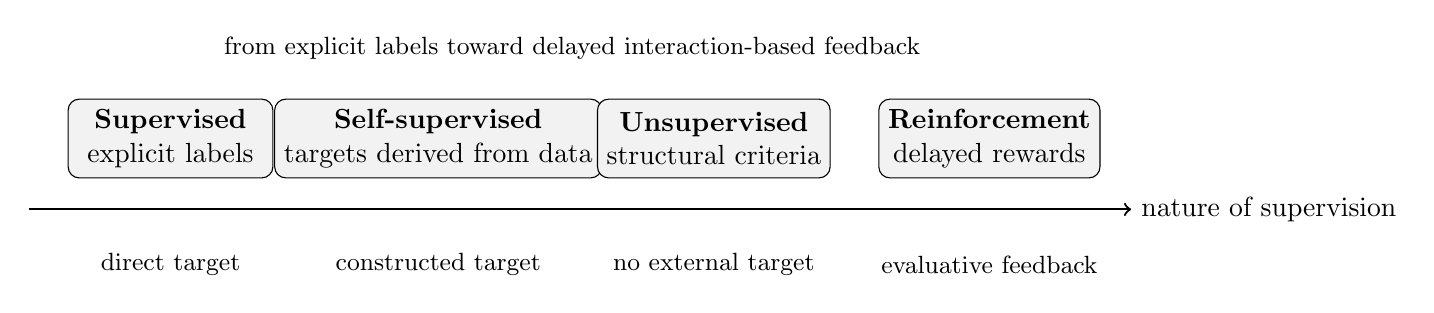
\begin{tikzpicture}[scale=1, every node/.style={align=center}]
    \draw[->, thick] (0,0) -- (14,0) node[right] {nature of supervision};

    \node[draw, rounded corners, fill=gray!10, minimum width=2.6cm, minimum height=1cm] (sup) at (1.8,0.9) {\textbf{Supervised}\\explicit labels};
    \node[draw, rounded corners, fill=gray!10, minimum width=2.8cm, minimum height=1cm] (self) at (5.2,0.9) {\textbf{Self-supervised}\\targets derived from data};
    \node[draw, rounded corners, fill=gray!10, minimum width=2.7cm, minimum height=1cm] (unsup) at (8.7,0.9) {\textbf{Unsupervised}\\structural criteria};
    \node[draw, rounded corners, fill=gray!10, minimum width=2.8cm, minimum height=1cm] (rl) at (12.2,0.9) {\textbf{Reinforcement}\\delayed rewards};

    \node at (1.8,-0.7) {\small direct target};
    \node at (5.2,-0.7) {\small constructed target};
    \node at (8.7,-0.7) {\small no external target};
    \node at (12.2,-0.7) {\small evaluative feedback};

    \node at (6.9,2.05) {\small from explicit labels toward delayed interaction-based feedback};
\end{tikzpicture}
\caption{The main paradigms can be arranged by the form of supervision they provide: from explicit labels, through internally constructed targets and structural objectives, to delayed rewards from interaction.}
\end{figure}

\subsection*{A comparative summary}

\begin{table}[tbp]
\centering
\renewcommand{\arraystretch}{1.25}
\begin{tabular}{p{2.2cm}p{2.3cm}p{2.6cm}p{2.8cm}p{2.6cm}}
\toprule
\textbf{Paradigm} & \textbf{Data} & \textbf{Supervision signal} & \textbf{Objective} & \textbf{Output / evaluation} \\
\midrule
Supervised
& labeled pairs $(x,y)$
& explicit external labels
& prediction loss
& predictor; accuracy, risk, error \\
\addlinespace
Unsupervised
& unlabeled inputs $x$
& structural regularities in data
& likelihood, reconstruction, clustering, compression
& representation or generative structure; likelihood, distortion, clustering quality \\
\addlinespace
Self-supervised
& unlabeled inputs $x$
& targets derived from the data
& auxiliary predictive objective
& representation or predictor; transfer quality, downstream performance \\
\addlinespace
Reinforcement
& trajectories $(s_t,a_t,r_t)$
& delayed reward from interaction
& expected cumulative reward
& policy; return, success rate, long-term performance \\
\bottomrule
\end{tabular}
\caption{A comparison of the main learning paradigms by data source, supervision signal, objective, output, and evaluation.}
\end{table}

\subsection*{Why the paradigms matter}

The paradigms are not merely administrative categories. They reflect genuinely different ways in which information can constrain learning.

\begin{itemize}
    \item Supervised learning asks how input-output relationships can be inferred from labeled examples.
    \item Unsupervised learning asks what structure can be extracted from observations alone.
    \item Self-supervised learning asks how raw data can be turned into their own supervisory signal.
    \item Reinforcement learning asks how action can be improved when feedback is delayed and shaped by interaction.
\end{itemize}

At the same time, the boundaries are not absolute. A modern system may pretrain representations self-supervisedly, fine-tune them with supervision, and then adapt them inside a reinforcement-learning loop. The paradigms are best understood as organizing viewpoints, not sealed compartments.

\whattoremember{The main learning paradigms differ by their supervision regime: supervised learning uses explicit labels, unsupervised learning uses structural criteria on unlabeled data, self-supervised learning creates targets from the data themselves, and reinforcement learning improves behavior through delayed rewards from interaction. Despite these differences, all four can be viewed as optimizing objective functionals over data or trajectories. The key unifying question is not whether there is an objective, but what form of information defines it.}

\subsection*{Exercises}

\begin{exercise}
For each of the following, identify the most natural learning paradigm and briefly justify your answer:
\begin{enumerate}
    \item predicting house prices from past sales data,
    \item grouping customers into behavioral segments without labels,
    \item predicting a masked word in a sentence,
    \item learning to control a robot arm from reward signals,
    \item reconstructing an image from a compressed latent code.
\end{enumerate}
\end{exercise}

\begin{exercise}
Write a toy self-supervised objective for one of the following settings:
\begin{enumerate}
    \item a sentence with one hidden token,
    \item an image with one missing patch,
    \item a time series with a short future segment to be predicted.
\end{enumerate}
Be explicit about what serves as the input and what serves as the target.
\end{exercise}

\begin{exercise}
Explain why reinforcement learning is not simply supervised learning on a dataset of trajectories. In your answer, discuss at least two of the following: delayed reward, exploration, action-dependent data, and long-term consequences.
\end{exercise}

\begin{exercise}
Give one example of an unsupervised objective and one example of a self-supervised objective. Why is it helpful to distinguish these two regimes instead of merging them into a single category?
\end{exercise}

\begin{exercise}
A modern model is pretrained by predicting missing tokens on a large text corpus and then fine-tuned on labeled sentiment examples. Which paradigms appear in this pipeline, and what role does each one play?
\end{exercise}

\subsection*{Notes and references}

The purpose of this section is to organize the major learning paradigms by the form of supervision they use while keeping a unified mathematical viewpoint. The crucial point is that the absence of explicit labels does not imply the absence of an objective. Unsupervised learning, self-supervised learning, and reinforcement learning all optimize structured criteria, but those criteria arise from different sources: data geometry, automatically constructed prediction tasks, or delayed evaluative feedback from interaction. This broader view will be important later when the book moves from classical supervised prediction to representation learning, generative modeling, and sequential decision-making.